\section{Signalling}
Signalling games involve choices of a party (sender) influencing the \impt{beliefs}, and therefore, actions of other parties (receivers). \\
The sender knows its own characteristic, and makes a public decision (signal). \\
The receiver is interested in the underlying characteristic. It observes the signal (which it may or may not care). \\
The model is described in the following way. Consider a sender (1) and a receiver, where S observes type $\theta \in \Theta$ (we can assume the types are distributed with probability density $p(\theta) \in [0, 1]$) that is exogenous. S chooses an action $a_1 \in A_1$, and R observes $a_1$ to choose $a_2 \in A_2$. The payoff for player $i$ is $u_i(a_1, a_2, \theta)$. \\
A pure strategy form $(s_1, s_2)$ is the mapping where $s_1: \Theta \to A_1$ and $s_2: A_1 \to A_2$. A mixed strategy form is described to be $\sigma_1(a_1 \mid \theta) = \prob(a_1 \mid \theta)$ and $\sigma_2(a_2 \mid a_2) = \prob(a_2 \mid a_1)$. The beliefs is a function that $\mu: A_1 \to \Delta(\Theta)$. For example, $\mu(\theta \mid a_1)$ represents the probability assigned to type $\theta$ by the receiver once action $a_1$ has been observed.
\begin{definition}
    A \uimpt{weak perfect Bayesian equilibrium} satisfies two conditions:
    \begin{quote}
        1. Rationality condition: players choose optimal strategies given beliefs. \\
        2. Consistency condition: beliefs are updated according to Bayes' rule.
    \end{quote}
    A pure strategy wPBE is $(s_1^*, s_2^*, \mu)$ satisfying sequential rationality for S and R:
    $$\forall \theta \in \Theta, s_1^*(\theta) \in \argmax_{a_1 \in A_1} u_1(a_1, s_2^*(a_1), \theta)$$
    $$\forall a_1 \in A_1, s_2^*(a_1) \in \argmax_{a_2 \in A_2} \Sumi{\theta} \mu^*(\theta \mid a_1) u_2(a_1, a_2, \theta)$$
    and Bayes Consistency
    $$\mu(\theta \mid a_1) = \begin{cases}
        \frac{\prob(\theta)}{\prob(a_1)} & s_1(\theta) = a_1 \\
        0 & s_1(\theta) \ne a_1
    \end{cases}$$
    where $\prob(a_1) = \Sumi{\{\theta' \mid s_1(\theta') = a_1\}} \prob(\theta')$
\end{definition}

\subsection{Spencer's Education Model}
Consider a sender to be a worker, and a receiver to be an employer. $A_1 = \R^+$ which indicates the education level, and $\Theta = \{L, H\}$ which indicates the productivity level. $A_2 = \R^+$ is the set of wages offered to the worker. \\
The payoffs are $u_1(a_1, a_2, \theta) = a_2 - \frac{a_1}{\theta}$ and $u_2(a_1, a_2, \theta) = -(a_2 - \theta)^2$. \\
There are three types of equilibrium: separating, pooling, and semi-pooling.
A separating equilibrium is when the sender chooses distinct actions according to their types. This means their actions are fully revealing. \\
A pooling equilibrium is when the sender chooses the same action regardless of their type, which conveys no information. \\
For this specific model, we start by analyzing the sequential rationality condition of player $2$.
\begin{align*}
    s_2(a_1) &= \Sumi{\theta} \mu(\theta \mid a_1)u_2(a_1, a_2, \theta) \\
    &= \mu(L \mid a_1)(-(a_2 - L)^2) + \mu(H \mid a_1)(-(a_2 - H)^2)
\end{align*}
To maximize, we take the first-order condition, and we have:
\begin{align*}
    \dv{a_2}s_2 &= -2\mu(L \mid a_1)(a_2 - L) - 2\mu(H \mid a_1)(a_2 - H) = 0 \\
    a_2^* &= \mu(L \mid a_1)L + \mu(H \mid a_1)H
\end{align*}
Then, we analyze the sequential rationality of player $1$. \\
If it is a separating equilibrium, and player $1$ plays $(a_L^*, a_H^*)$ respectively when its type is $(L, H)$, then $s_2(a_L^*) = L$ and $s_2^*(a_H^*) = H$.
\begin{quote}
    We want to make sure that when it is L type, it has no incentive to deviate, that is
    $$u_1(a_L^*, L, L) \ge u_1(a_1, s_2^*(a_1), L)$$
    when $a_1 = 0$, this gives that $L - \frac{a_L^*}{L} \ge s_2(0) - \frac{0}{L} \ge L$, which means $a_L^* = 0$. \\
    We also want to ensure that if it is L type, it has no incentive to pretend it is H type
    $$u_1(a_L^* = 0, L, L) \ge u_1(a_H^*, H, L)$$
    and when it is H type, it has no incentive to pretend it is L type
    $$u_1(a_L^* = 0, L, H) \le u_1(a_H^*, H, H)$$
    These two solve to $(H-L)L \le a_H^* \le (H-L)H$. \\
    This means, a separating wPBE with the given choices exists if and only if $a_L^* = 0$ and $a_H^*$ satisfies the derived condition.
\end{quote}
It is already shown that if there exists a separating equilibrium, the above condition holds, however, we also need to show that if the condition holds, there exists a separating equilibrium. In this case, there are cases where the Bayesian beliefs cannot be updated (e.g. $a_1 \ne a_L^*, a_H^*$). We just say the employer assumes the worst and $\mu(H \mid a_1) = 0$ in these cases. If we write out all the beliefs and strategies of player $2$, we can find the payoff for player $1$ when it is L, is always $0$; and when it is H, is $H - \frac{a_H^*}{H}$. The least-cost separating equilibrium is Pareto dominant, that is $a_H^* = (H-L)L$. \\
\bigskip \\
If it is a pooling equilibrium, that is $s_1^*(H) = s_1^*(L) = a^*$, then $\mu(H \mid a_1) = \prob(H)$. The sequential rationality condition for player $2$ is:
$$\bar{\theta} := \prob(H)H + \prob(L)L$$
Deviating to $a_1 = 0$ must not be profitable for player $1$:
$$\bar{\theta} - \frac{a^*}{\theta} \ge s_2(0) - \frac{0}{\theta} \ge L$$
this means that $a^* \le (\bar{\theta} - L)\theta$. A pooling equilibrium with signal $a^*$ exists if and only if $a^* \le (\bar{\theta} - L)L$. A complete equilibrium is described by $(s_1^*(\theta), s_2^*(a_1), \mu)$.

\subsection{Intuitive Criterion}
First [\dots] given the equilibrium outcome, a given out of equilibrium message is not sensible for certain type of [sender]. Second, insofar as this asserted fact is held by the players to be correct, introspection on their part will them that [receiver] will attach zero weight to this out-of-equilibrium message coming from those types [\dots]. A wPBE satisfies the intuitive criterion if the equilibrium belief $\mu^*$ is consistent with the intuitive logic. In the Spencer's model, this means three things:
\begin{quote}
    1. If the intuitive criterion is satisfied, we must have
    $$\mu(H \mid a_1) = 1, \forall a_1 \in (\underbar{a}_H, a_H^*)$$
    2. This cannot be the case in equilibrium since H types would want to deviate from $a_H^*$ to $a_1$, since employers would pay H to all education levels $a_1 \in (\underbar{a}_H, a_H^*]$. \\
    3. The only separating equilibrium satisfying the intuitive criterion is the least-cost separating equilibrium.
\end{quote}
This is saying: if type L is clearly not attracted by education $a$, but type H potentially attracted, then a receiver would conclude that $a$ has been chosen by type H. To be clearly not attracted by $a$, type L would not choose $a$ even with the highest possible reward; to be potentially attracted by $a$, the highest possible reward would attract type H to choose $a$.

\subsection{Beer-Quiche Game}
Consider a game described as the following extensive form:
\begin{center}
    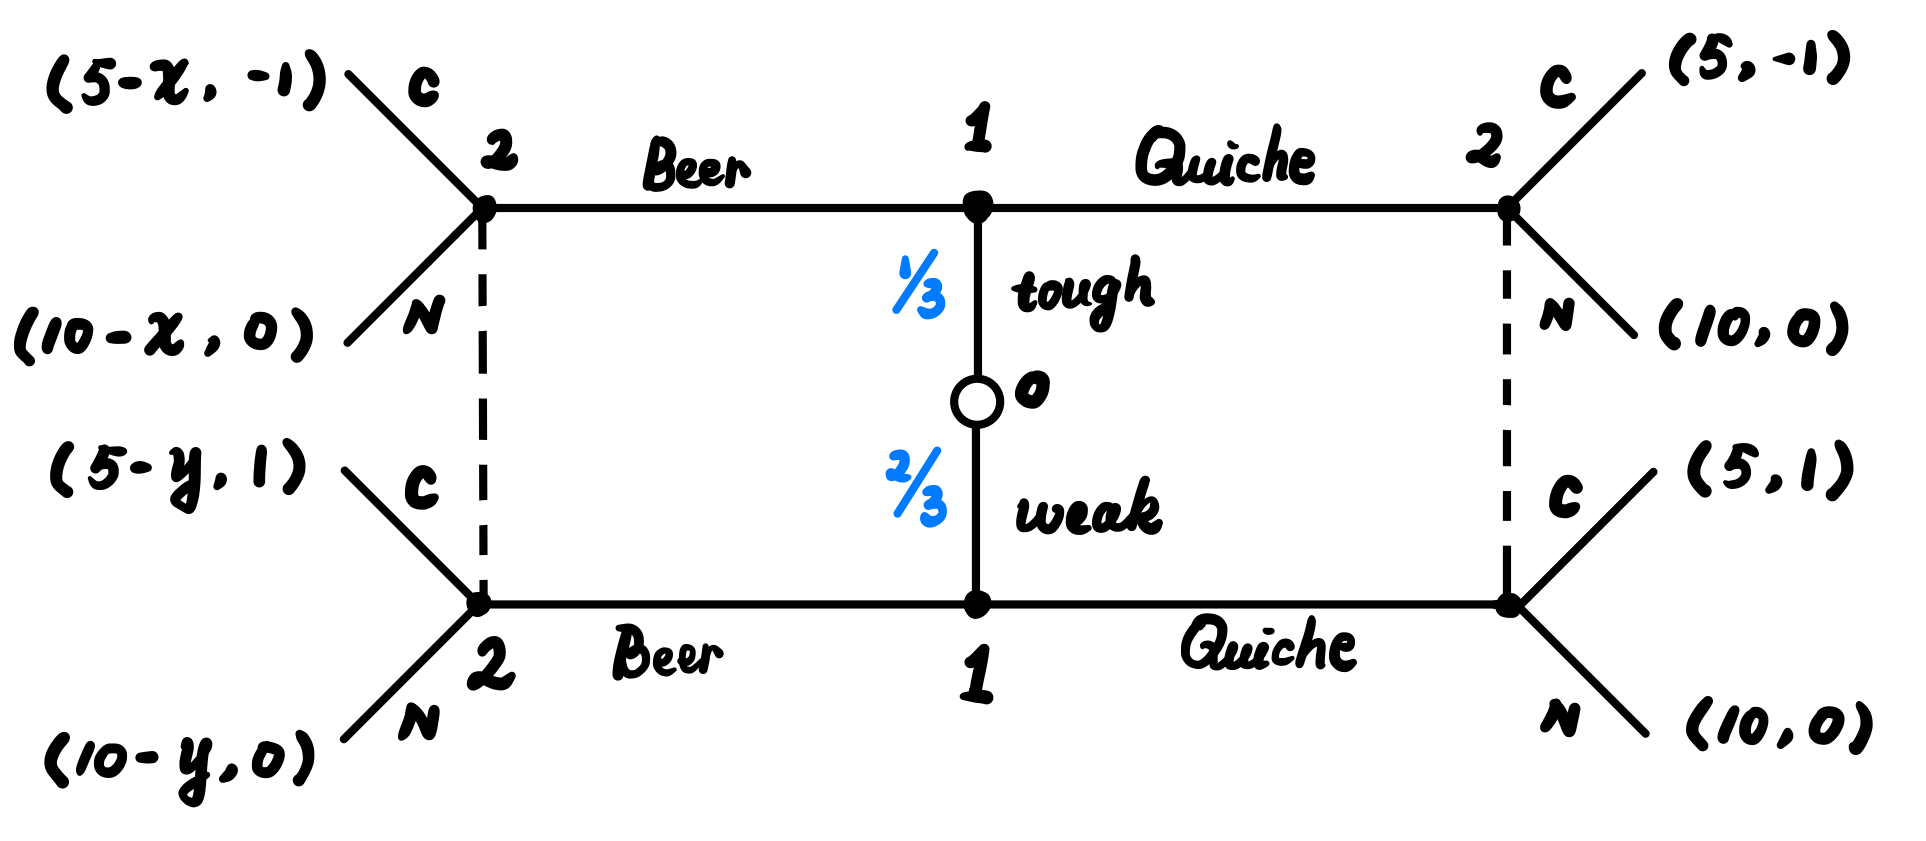
\includegraphics[scale = 0.2]{4/beer-quiche.png}
\end{center}
where $x, y > 0$ and C means challenge and N means not challenge. \\
We start by looking at player $2$'s sequential rationality:
\begin{quote}
    1. If player $2$ decides to challenge given $a_1 = K \in \{B, Q\}$, then
    $$U_2(C \mid K) = \mu_K(-1) + (1-\mu_k)(1) = 1 - 2\mu_K$$
    where $\mu_K = \mu(T \mid K)$. \\
    2. $U_2(N \mid K)  = 0$. \\
    In equilibrium, player $2$'s best response is:
    $$a_T = \begin{cases}
        C & \mu_K < \frac{1}{2} \\
        N & \mu_K > \frac{1}{2} \\
        \text{indifferent} & \mu_K = \frac{1}{2}
    \end{cases}$$
\end{quote}
Then, we look at player $1$'s sequential rationality. \\
First consider $a_T = a_W = B$, this gives $\mu_B = \frac{1}{3}$ which leads to $a_B = C$. Then $U_1(B \mid W) = 5 - y$ and $U_1(Q \mid W) = 5 \text{ or } 10$. Choosing Q is better than B for weak type, so this cannot be a pooling equilibrium. \\
Then consider $a_T = a_W = Q$, this gives $\mu_Q = \frac{1}{3}$, meaning that $a_Q = C$. The most convenient belief is that $\mu_B = 0$ and $a_B = C$ as well. In this case,
\begin{quote}
    $U_1(Q \mid W) = 5, U_1(B \mid W) = 5 - y$. \\
    $U_1(Q \mid T) = 5, U_1(B \mid T) = 5 - x$.
\end{quote}
This means, there is a pooling PBE in this case. \\
Furthermore, consider two types of separating PBE:
\begin{quote}
    1. $a_T = B, a_W = Q$: this gives that $\mu_B = 1$, and $\mu_Q = 0$. Player $2$ will play $a_B = N, a_Q = C$. We need to have
    \begin{align*}
        U_1(B \mid T) &\ge U_1(Q \mid T) \\
        10 - x &\ge 5 \\
        x &\le 5
    \end{align*}
    \begin{align*}
        U_1(B \mid W) &\le U_1(Q \mid W) \\
        10 - y &\le 5 \\
        y &\ge 5
    \end{align*}
    2. $a_T = Q, a_W = B$: this gives that $\mu_B = 0, \mu_Q = 1$. Player $2$ will play $a_B = C$ and $a_Q = N$. We need to have
    \begin{align*}
        U_1(B \mid T) &\le U_1(Q \mid T) \\
        5 - x &\le 10
    \end{align*}
    \begin{align*}
        U_1(B \mid W) &\ge U_1(Q \mid W) \\
        5 - y &\ge 10
    \end{align*}
    In this case, there cannot be a separating PBE. Only the first case stands.
\end{quote}
Finally, we discuss a semi-pooling PBE, where we need mixed strategies. We define that
$$\sigma_\theta = \prob(a_1 = B \mid \theta)$$
Then, we must have:
\begin{align*}
    \mu_B &= \mu(T \mid B) = \frac{\frac{1}{3}\sigma_T}{\frac{1}{3}\sigma_T + \frac{2}{3}\sigma_W} = \frac{\sigma_T}{\sigma_T + 2\sigma_W} \\
    \mu_Q &= \mu(T \mid Q) = \frac{\frac{1}{3}(1 - \sigma_T)}{\frac{1}{3}(1-\sigma_T) + \frac{2}{3}(1 - \sigma_W)} = \frac{1 - \sigma_T}{(1 - \sigma_T) + 2(1-\sigma_W)}
\end{align*}
We show that the semi-pooling equilibrium exists when $\sigma_T = 1$ and $\sigma_W \in (0, 1)$, and $\mu_B = \frac{1}{1 + 2\sigma_W}$, $\mu_Q = 0$. \\
Let $\alpha_K = \prob(a_2 = C \mid a_1 = K)$
Then player $1$ must have the indifference condition for weak type where
\begin{align*}
    U_1(Q \mid W) &= U_1(B \mid W) \\
    5 &= (5 - y)\alpha_B  + (10 -y)(1 - \alpha_B) \\
    \alpha_B &= 1-\frac{y}{5}
\end{align*}
However, this mix is optimal only if player $2$ is indifferent from its sequential rationality:
$$\mu_B = \frac{1}{1 + 2\sigma_W} = \frac{1}{2} \to \sigma_W = \frac{1}{2}$$
We finally check that optimality of type T:
$$U_1(B \mid T) \ge U_1(Q \mid T) \to \alpha_B(5 - x) + (1-\alpha_B)(10 - x) \ge 5$$
This gives that $y \ge x$.



\newpage